\nTitle{Analyse multicritère}

Des deux parties précedentes, emergent 8 propositions de gestion de l'atelier.
Le but de cette partie sera de selectionner la meilleure solution en fonction de 4 critères.

\subsection{Méthode choisie}

La méthode de résolution choisie sera Electre III car elle englobe les 2 précedentes.
On pourras ainsi fournir au client la méthode sélectionné comme la plus optimale ainsi qu'une ou plusieurs méthodes alternatives.

Pour réduire au maximum l'échéance, nous avons parallelisé au maximum les flux de travail.
Nous avons donc dès le début du projet commencé par coder sous MatLab un algorithme de résolution de Electre 3.

\subsection{Mise en œuvre de la méthode}

L'algorithme très simple est identique à la méthode proposé en cours :

à partir de la matrice des jugements, il remet à l'echelle les notes des critères en fonction des poids.

for i = 1:n
	J(:,i) = ( (J(:,i) - (e/2)) * (w(i)/max(w))) + (e/2);
end;

Puis il calcule les matrices de concordance et de discordance.

for i = 1:n
    for j = 1:n
        if (i ~= j)
            C(i,j) = sum( (J(i,:)>=J(j,:)).*w )/sum(w);
            D(i,j) = max(max(J(j,:)-J(i,:)),0)/e;
        end;
    end;
end;

Pour finir, il établit la matrice des surclassement en fonction de ces deux dernières matrices.

S = ((C > s).*(D <= v));

Un graph est ensuite généré à partir de cette matrice.
On obtient ainsi rapidement la meilleurs solution en tête de graphe, et grace à la méthode du classement et du classement inverse, on peut obtenir l'ordre des solutions.

\subsection{Solution proposé}

Dans un premier temps, sans prendre en compte l'étude des 2 première parties, la meilleur solution, serait la solution A.

\begin{figure}
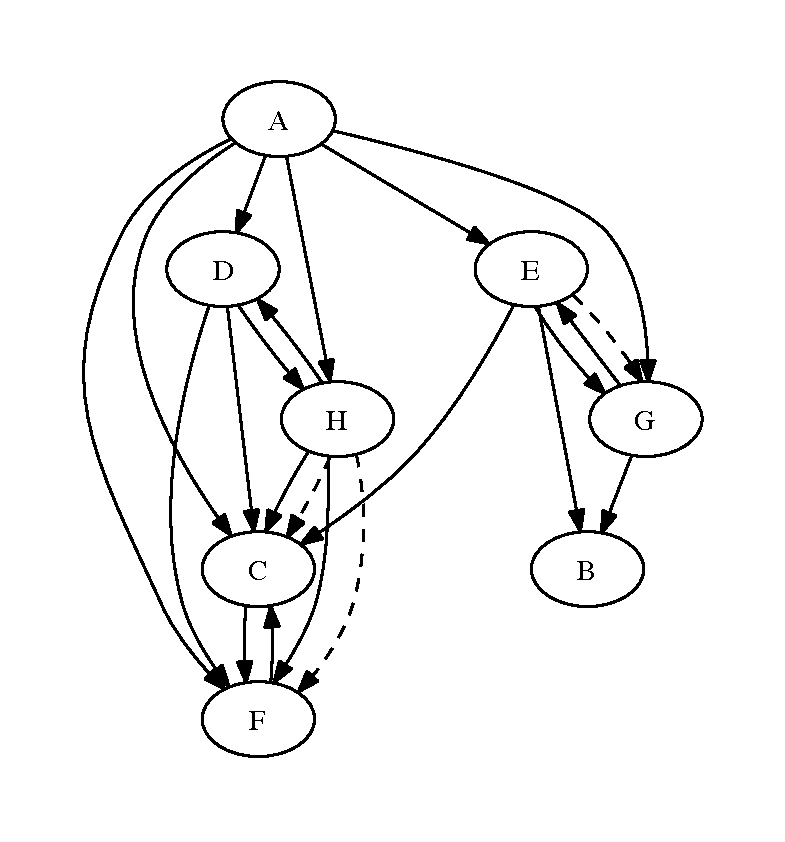
\includegraphics{../SourcesMatlab/electre3-1.pdf}
\caption{Graphe des surclassement sans prise en compte des poids de chaque critère}
\end{figure}

Dans un second temps, en prenant en compte les poids apporté par l'étude des 2 première parties.
